

%\documentclass[11pt, oneside]{article}   	
%\usepackage{geometry}    
%\geometry{letterpaper}                 		
\input preamble.tex
\newcommand{\ig}[2][width=4in]{\includegraphics[#1]{#2}}    		
\usepackage{graphicx}					
\usepackage{amssymb}
\usepackage{pgfplotstable}
\begin{document}

\header {\today}							
\title{Relativistic Electron Momentum}
\author{Ekta Patel \& Brandon Booth-Dunbar}



\section{Abstract}
\begin{em}
%Brandon
\end{em}

\section{Intro}
%Brandon

\section{Theory}
%Ekta

Using relativistic energy and momentum:

\begin{equation} E=m_0c^2+KE=\gamma mc^2\end{equation}
\begin{equation} p=\gamma v^2\end{equation}
\begin{equation}E^2=p^2c^2+m^2c^4\end{equation}
\begin{equation}KE+mc^2=\sqrt{p^2c^2+m^2c^4}\end{equation}
We know KE from the lab manual in units of MeV, solve for p:
\begin{equation}(KE+mc^2)^2=p^2c^2+m^2c^4\end{equation}
\begin{equation}(KE+mc^2)^2-m^2c^4=p^2c^2\end{equation}
\begin{equation}\frac{(KE+mc^2)^2-m^2c^4}{c^2}=p^2\end{equation}
\begin{equation}\frac{p=\sqrt{(KE+mc^2)^2-m^2c^4}}{c}\end{equation}
We are given:
\begin{equation}p=qRB\end{equation}
Where R is the radius of the detector-source apparatus, which we have measured to be .0290m:
\begin{equation}\frac{p=\sqrt{(KE+mc^2)^2-m^2c^4}}{c}=eB(.0290m)\end{equation}
Solving for B, we can estimate our magnetic fields needed to see the electron pulses:
\begin{equation}B=\frac{\sqrt{(KE+mc^2)^2-m^2c^4}}{ce(.0290m)}\end{equation}
Before solving for B, we must account for the energy lost by the electron due to k-shell binding energy which is $\sim$88keV:
\begin{equation}KE=1.064MeV-0.088005MeV=0.975995\end{equation}
Now, we can substitute all of our values into equation 11 to obtain:
\begin{equation} B=0.1606T=1.606kG\end{equation}
For the second electron pulse with .5689MeV:
\begin{equation}KE=0.5689MeV-.0.088005MeV=MeV\end{equation}
Once again, using equation 11:
\begin{equation}B=0.0979T=0.979kG\end{equation}

Remember to consider the fact that the electron loses energy as it travels in the air when doing error analysis!

\section{Experimental Methods}
%Brandon
\subsection{Apparatus}

\subsection{Calibration}
The calibration of the apparatus is the most detail sensitive step in the experiment.  While calibrating the detector system if you set the amplifier too high or the single channel analyzer too low you will get very large background counts from the sensor and willnot reliably be able to detect the peaks of electron emission from the �Byzanthium? source.  On the other hand if the discriminator is set too high or the amplifier to low you will not get enough counts to clearly define a peak when you perform your measurements. 
\subsection{Procedure}

\section{Results $\&$ Discussion}
%Ekta

\section{Conclusion}
%Ekta & Brandon

\section{Appendix}
Data tables and graphs.

\begin{table}
\caption{Run 1}
\begin{tabular}{|c|c|c|} \hline
Field	(kG)&	Counts	&	Error	\\	\hline
0.6009	&	10	&	3.16	\\	\hline
0.6500	&	26	&	5.10	\\	\hline
0.7009	&	20	&	4.47	\\	\hline
0.7505	&	25	&	5.00	\\	\hline
0.8008	&	32	&	5.66	\\	\hline
0.8507	&	28	&	5.29	\\	\hline
0.9006	&	35	&	5.92	\\	\hline
0.9503	&	44	&	6.63	\\	\hline
1.0002	&	36	&	6.00	\\	\hline
1.0525	&	51	&	7.14	\\	\hline
1.1067	&	40	&	6.32	\\	\hline
1.1498	&	18	&	4.24	\\	\hline
1.2000	&	27	&	5.20	\\	\hline
1.2546	&	31	&	5.57	\\	\hline
1.3061	&	29	&	5.39	\\	\hline
1.3528	&	22	&	4.69	\\	\hline
1.4012	&	20	&	4.47	\\	\hline
1.4503	&	25	&	5.00	\\	\hline
1.5016	&	41	&	6.40	\\	\hline
1.5526	&	50	&	7.07	\\	\hline
1.6018	&	79	&	8.89	\\	\hline
1.6512	&	101	&	10.05	\\	\hline
1.7022	&	74	&	8.60	\\	\hline
1.7554	&	61	&	7.81	\\	\hline
1.8021	&	40	&	6.32	\\	\hline
1.8524	&	24	&	4.90	\\	\hline
1.9022	&	20	&	4.47	\\	\hline
1.9495	&	27	&	5.20	\\	\hline
2.0010	&	15	&	3.87	\\	\hline
\end{tabular}
\end{table}

\begin{table}
\caption{Run 2}
\begin{tabular}{|c|c|c|} \hline
Field	&	Counts	&	Error	\\ \hline
0.6009	&	14	&	3.74	\\ \hline
0.6500	&	17	&	4.12	\\ \hline
0.7004	&	21	&	4.58	\\ \hline
0.7520	&	21	&	4.58	\\ \hline
0.8014	&	33	&	5.74	\\ \hline
0.8502	&	25	&	5.00	\\ \hline
0.9025	&	37	&	6.08	\\ \hline
0.9505	&	36	&	6.00	\\ \hline
1.0002	&	41	&	6.40	\\ \hline
1.0525	&	38	&	6.16	\\ \hline
1.1004	&	33	&	5.74	\\ \hline
1.1501	&	33	&	5.74	\\ \hline
1.2017	&	29	&	5.39	\\ \hline
1.2506	&	21	&	4.58	\\ \hline
1.3006	&	26	&	5.10	\\ \hline
1.3509	&	35	&	5.92	\\ \hline
1.4012	&	19	&	4.36	\\ \hline
1.4506	&	30	&	5.48	\\ \hline
1.5030	&	39	&	6.24	\\ \hline
1.5497	&	60	&	7.75	\\ \hline
1.6015	&	84	&	9.17	\\ \hline
1.6531	&	92	&	9.59	\\ \hline
1.7008	&	80	&	8.94	\\ \hline
1.7535	&	66	&	8.12	\\ \hline
1.8009	&	58	&	7.62	\\ \hline
1.8501	&	36	&	6.00	\\ \hline
1.9009	&	29	&	5.39	\\ \hline
1.9510	&	22	&	4.69	\\ \hline
2.0019	&	16	&	4.00	\\ \hline
\end{tabular}
\end{table}

\begin{table}
\caption{Run 3}
\begin{tabular}{|c|c|c|} \hline
Field	&	Counts	&	Error	\\ \hline
0.6006	&	19	&	4.36	\\ \hline
0.6496	&	20	&	4.47	\\ \hline
0.7028	&	27	&	5.20	\\ \hline
0.7513	&	26	&	5.10	\\ \hline
0.8015	&	17	&	4.12	\\ \hline
0.8508	&	22	&	4.69	\\ \hline
0.9008	&	30	&	5.48	\\ \hline
0.9509	&	53	&	7.28	\\ \hline
1.0015	&	31	&	5.57	\\ \hline
1.0498	&	36	&	6.00	\\ \hline
1.1000	&	42	&	6.48	\\ \hline
1.1508	&	30	&	5.48	\\ \hline
1.2014	&	24	&	4.90	\\ \hline
1.2508	&	35	&	5.92	\\ \hline
1.3047	&	16	&	4.00	\\ \hline
1.3518	&	29	&	5.39	\\ \hline
1.4011	&	22	&	4.69	\\ \hline
1.4515	&	33	&	5.74	\\ \hline
1.5027	&	41	&	6.40	\\ \hline
1.5505	&	67	&	8.19	\\ \hline
1.6025	&	88	&	9.38	\\ \hline
1.6518	&	92	&	9.59	\\ \hline
1.7015	&	81	&	9.00	\\ \hline
1.7518	&	50	&	7.07	\\ \hline
1.8043	&	40	&	6.32	\\ \hline
1.8519	&	14	&	3.74	\\ \hline
1.9020	&	23	&	4.80	\\ \hline
1.9514	&	21	&	4.58	\\ \hline
2.0021	&	14	&	3.74	\\ \hline
\end{tabular}
\end{table}

\begin{table}
\caption{Run 4}
\begin{tabular}{|c|c|c|} \hline
Field (kG)	&	Counts	&	Error	\\ \hline
2.0024	&	25	&	5.00	\\ \hline
1.9532	&	25	&	5.00	\\ \hline
1.9019	&	25	&	5.00	\\ \hline
1.8519	&	34	&	5.83	\\ \hline
1.8253	&	29	&	5.39	\\ \hline
1.8006	&	40	&	6.32	\\ \hline
1.7750	&	58	&	7.62	\\ \hline
1.7503	&	55	&	7.42	\\ \hline
1.7251	&	74	&	8.60	\\ \hline
1.7009	&	94	&	9.70	\\ \hline
1.6902	&	92	&	9.59	\\ \hline
1.6801	&	93	&	9.64	\\ \hline
1.6701	&	105	&	10.25	\\ \hline
1.6603	&	122	&	11.05	\\ \hline
1.6505	&	100	&	10.00	\\ \hline
1.6001	&	92	&	9.59	\\ \hline
1.5903	&	83	&	9.11	\\ \hline
1.5805	&	92	&	9.59	\\ \hline
1.5705	&	69	&	8.31	\\ \hline
1.5602	&	75	&	8.66	\\ \hline
1.5517	&	72	&	8.49	\\ \hline
1.5254	&	45	&	6.71	\\ \hline
1.5038	&	33	&	5.74	\\ \hline
1.4759	&	29	&	5.39	\\ \hline
1.4507	&	27	&	5.20	\\ \hline
1.4249	&	35	&	5.92	\\ \hline
1.4019	&	33	&	5.74	\\ \hline
1.3514	&	20	&	4.47	\\ \hline
1.3035	&	36	&	6.00	\\ \hline
1.2501	&	26	&	5.10	\\ \hline
1.2041	&	28	&	5.29	\\ \hline
1.1528	&	20	&	4.47	\\ \hline
1.1255	&	39	&	6.24	\\ \hline
1.1027	&	32	&	5.66	\\ \hline
1.0896	&	34	&	5.83	\\ \hline
1.0805	&	43	&	6.56	\\ \hline
1.0702	&	47	&	6.86	\\ \hline
1.0606	&	42	&	6.48	\\ \hline
1.0509	&	41	&	6.40	\\ \hline
1.0246	&	43	&	6.56	\\ \hline
1.0011	&	39	&	6.24	\\ \hline
0.9531	&	39	&	6.24	\\ \hline
0.9050	&	43	&	6.56	\\ \hline
0.8511	&	30	&	5.48	\\ \hline
0.8022	&	40	&	6.32	\\ \hline
0.7521	&	21	&	4.58	\\ \hline
0.7020	&	28	&	5.29	\\ \hline
0.6498	&	20	&	4.47	\\ \hline
0.6004	&	26	&	5.10	\\ \hline
\end{tabular}
\end{table}

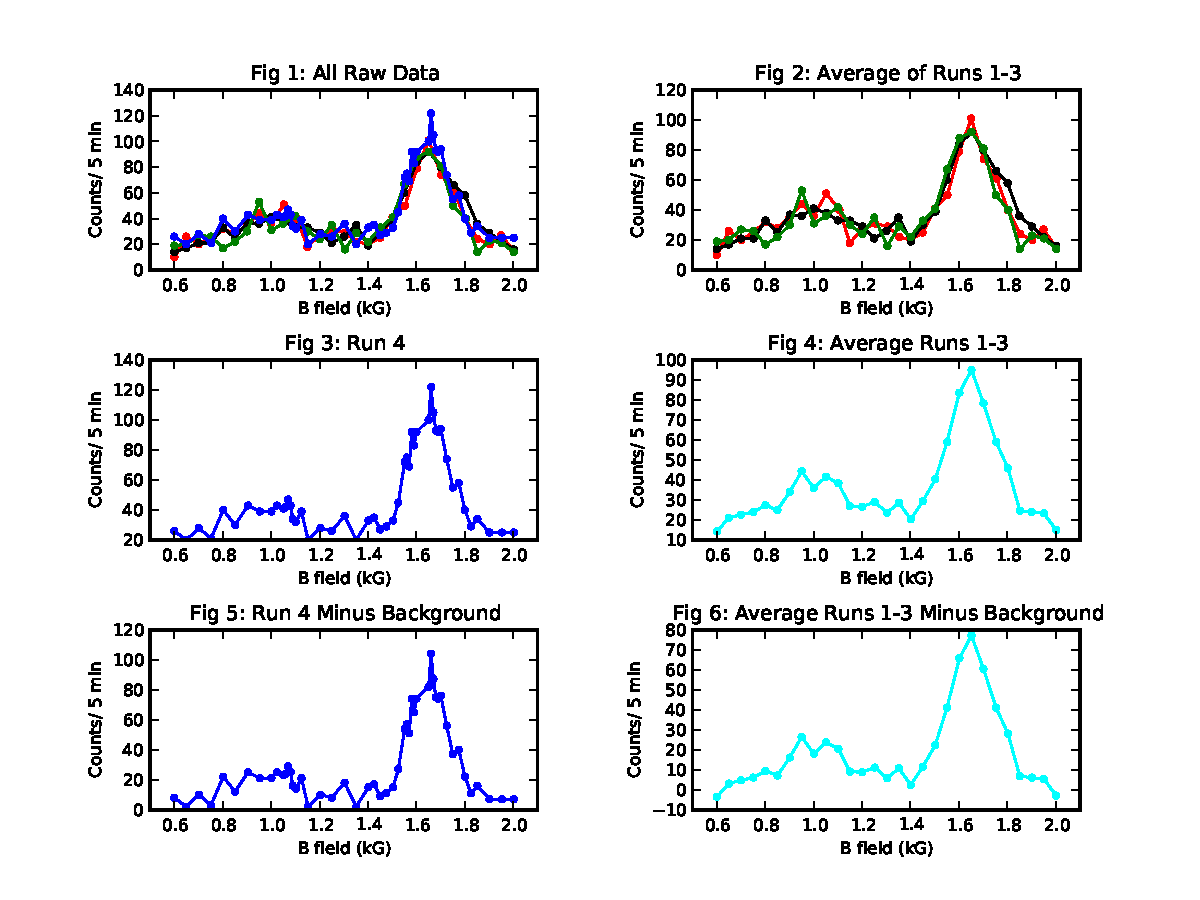
\includegraphics[width=7.5in]{field_counts.pdf}

%\pgfplotstabletypeset[columns={[index]0,[index]1}, precision=4]{data.txt}
%Referenecs
%Appendix



\end{document}  
